\chapter{Design og implementering}


\section{Software Design}

\subsection{Modultest}



\section{Hardware Design}
På baggrund af BDD'et er der fundet følgende hardwareblokke, der skal udarbejdes: 
\begin{itemize}
	\item Motorstyring
	\item Tre motorer
\end{itemize}

\subsection{Motorstyring}
Til at styre de tre motorer er der bygget en H-bro, der skal bruges i tre eksemplarer. To af disse motorer skal kunne styre kanonen, så den kan køre op og ned og frem og tilbage. Den tredje skal bruges til at styre affyringsekanismen. 

\subsubsection{H-bro}
Først blev der designet en H-bro, som bestod af to N-MOSFET's af typen IRLZ44 og to P-MOSFET's af typen ZVP3306. Denne kan ses på figur... Det viste sig dog, at den P-MOSFET der var brugt, var for svag til at kunne trække den strøm, som motoren skulle bruge, hvilket betød, at den blev brændt af. 


\begin{figure}[H]
	\centering
	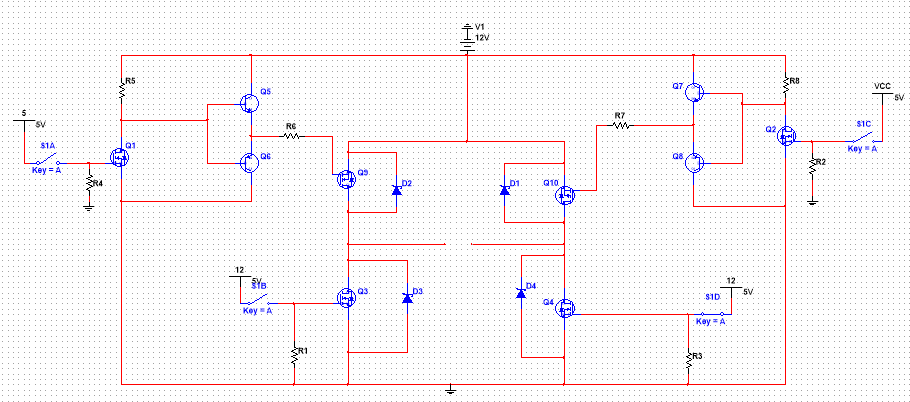
\includegraphics[]{DesignOgImplementering/images/motorkreds}
	\caption{H-bro kredsløb}
	\end{figure}

\begin{table}[]
	\centering
	\caption{Komponentbetegnelser på H-bro}
	\label{my-label}
	\begin{tabular}{|l|l|l}
		\cline{1-2}
		Betegnelse 	& Komponent 	          	 &  \\ \cline{1-2}
		VCC        	& 5V                         &  \\ \cline{1-2}
		Q1   		& IRLZ44(mosfet N-Channel)   &  \\ \cline{1-2}
		Q2   		& IRLZ44(mosfet N-Channel)   &  \\ \cline{1-2}
		Q3   		& IRLZ44(mosfet N-Channel)   &  \\ \cline{1-2}
		Q4   		& IRLZ44(mosfet N-Channel)   &  \\ \cline{1-2}
		Q5   		& BC547                      &  \\ \cline{1-2}
		Q6   		& BC557                      &  \\ \cline{1-2}
		Q7   		& BC547                      &  \\ \cline{1-2}
		Q8   		& BC557                      &  \\ \cline{1-2}
		Q9   		& IRF9Z34N(mosfet P-Channel) &  \\ \cline{1-2}
		Q10  		& IRF9Z34N(mosfet P-Channel) &  \\ \cline{1-2}
		R1   		& 10k$\Omega$                &  \\ \cline{1-2}
		R2   		& 10k$\Omega$                &  \\ \cline{1-2}
		R3   		& 10k$\Omega$                &  \\ \cline{1-2}
		R4   		& 10k$\Omega$                &  \\ \cline{1-2}
		R5   		& 10k$\Omega$                &  \\ \cline{1-2}
		R6   		& 100$\Omega$                &  \\ \cline{1-2}
		R7   		& 100$\Omega$                &  \\ \cline{1-2}
		R8   		& 10k$\Omega$                &  \\ \cline{1-2}
		D1   		& IN5819                     &  \\ \cline{1-2}
		D2   		& IN5819                     &  \\ \cline{1-2}
		D3   		& IN5819                     &  \\ \cline{1-2}
		D4   		& IN5819                     &  \\ \cline{1-2}
	\end{tabular}
\end{table}

\subsubsection{Mosfet}
Til at styre motor er der blevet bygget en H-bro, som består af fire mosfet, hvor to af dem er af typen  IRF9Z34N(mosfet P-channel, som er Q9 og Q10 på kredsløbs terningen ) og de to andre mosfet er af typen IRLZ44(mosfet N-Channel, som er Q3 og Q4 kredsløbs terningen). Der er blevet valgt at bruge mosfet for at kunne styre H-broen, for der kan man lukker og åbne for spændingen og de bliver styret af spænding, i forhold til transistor som bliver styret med strøm.
\begin{itemize}
	\item Mosfet n channel:\\
	\item 
	Mosfet p channel: \\
	Den kan klare en strøm på 6.7A, ifølge databladet. Så det vil ikke komme til at påvirker motoren, som kan trække en strøm på 0.35A. 
	
	for at der kan løbe spænding igennem IRF9Z34N(mosfet P-channel), så skal den have en negativ spænding for at åben op og have en spæding på over 0V for at lukke. 
	
\end{itemize}
\subsubsection{Diode}
Over fire af mosfetene(Q9,Q10,Q3 og Q4) er der blevet sat en diode af typen IN5819, den skal fungerer som beskyttelse af de fire mosfet(Q9,Q10,Q3 og Q4). Det de gør er at de sikre at den spænding, som er tilbage i motoren, når man lukker for mosfetene, ikke løber tilbage ind i mosfetene og brænder dem af.

\subsubsection{Modstande}
\begin{itemize}
	\item Pull down modstande:\\
	Der er blevet brugt fire modstande(R1,R2,R3 og R4), som pull down modstande, som søger for at signalet vil blive holdt lavet når der ikke er trykket, så det ben ikke står og flyver, så det kan komme til at åbne en mosfet, ved fejl og der ved kommer til at brænde mosfet eller motor af.  Der er valgt en modstand på 10kOhm, som stor nok til at trække de små spændinger ned, når der ikke er trykket og den stor nok til at spændingen ikke løber der ned når der er trykket.
	\item modstande
	\begin{itemize}
		\item R6 og R7
		
		\item R5 og R8
	\end{itemize}
	
	
\end{itemize}
\subsubsection{Motor}